\documentclass[letterpaper]{sig-alternate}


\pdfpagewidth=8.5in
\pdfpageheight=11in

%\usepackage[factor=250,spacing=true]{microtype}

\begin{document}
\conferenceinfo{RecSys '14}{October 6--10, 2014, Foster City, Silicon Valley, USA}
%\CopyrightYear{2007} % Allows default copyright year (20XX) to be over-ridden - IF NEED BE.
%\crdata{0-12345-67-8/90/01}  % Allows default copyright data (0-89791-88-6/97/05) to be over-ridden - IF NEED BE.

\title{TODO: title}

\numberofauthors{2}

\author {
\alignauthor
Daniel Kluver\\
\affaddr{GroupLens Research}\\
\affaddr{Department of Computer Science and Engineering}\\
\affaddr{University of Minnesota}\\
\affaddr{Minneapolis, MN 55455 USA}\\
\email{kluver@cs.umn.edu}
\alignauthor
Joseph A. Konstan\\
\affaddr{GroupLens Research}\\
\affaddr{Department of Computer Science and Engineering}\\
\affaddr{University of Minnesota}\\
\affaddr{Minneapolis, MN 55455 USA}\\
\email{konstan@cs.umn.edu}
}

\maketitle
\begin{abstract}

TODO: abstract

\end{abstract}

%TODO: update these things.
% A category with the (minimum) three required fields
\category{H.4}{Information Systems Applications}{Miscellaneous}
%A category including the fourth, optional field follows...
\category{D.2.8}{Software Engineering}{Metrics}[complexity measures, performance measures]

%TODO: update these things.
\terms{Theory}

%TODO: update these things.
\keywords{ACM proceedings, \LaTeX, text tagging}

\section{Introduction}
\section{Methodology}
\section{Results}

\begin{figure}
\centering
\includegraphics[width=\columnwidth]{../lenskit/target/analysis/RMSE.pdf}
\caption{caption}
\label{fig:rmse}
\end{figure}

\begin{figure}
\centering
\includegraphics[width=\columnwidth]{../lenskit/target/analysis/nDCG.pdf}
\caption{caption}
\label{fig:ndcg}
\end{figure}

\begin{figure}
\centering
\includegraphics[width=\columnwidth]{../lenskit/target/analysis/MAP.pdf}
\caption{caption}
\label{fig:map}
\end{figure}

\begin{figure}
\centering
\includegraphics[width=\columnwidth]{../lenskit/target/analysis/Precision.pdf}
\caption{caption}
\label{fig:precision}
\end{figure}

\begin{figure}
\centering
\includegraphics[width=\columnwidth]{../lenskit/target/analysis/Precision_fallout.pdf}
\caption{caption}
\label{fig:fallout}
\end{figure}

\begin{figure}
\centering
\includegraphics[width=\columnwidth]{../lenskit/target/analysis/TopN_RMSE_seenItems.pdf}
\caption{caption}
\label{fig:topn.rmse.seen}
\end{figure}

\begin{figure}
\centering
\includegraphics[width=\columnwidth]{../lenskit/target/analysis/TopN_RMSE.pdf}
\caption{caption}
\label{fig:topn.rmse}
\end{figure}

\begin{figure}
\centering
\includegraphics[width=\columnwidth]{../lenskit/target/analysis/TopN_Ave_Rat.pdf}
\caption{caption}
\label{fig:topn.avg.rat}
\end{figure}

\begin{figure}
\centering
\includegraphics[width=\columnwidth]{../lenskit/target/analysis/TopN_MeanPopularity.pdf}
\caption{caption}
\label{fig:pop}
\end{figure}

\begin{figure}
\centering
\includegraphics[width=\columnwidth]{../lenskit/target/analysis/diversity.pdf}
\caption{caption}
\label{fig:diversity}
\end{figure}

\begin{figure}
\centering
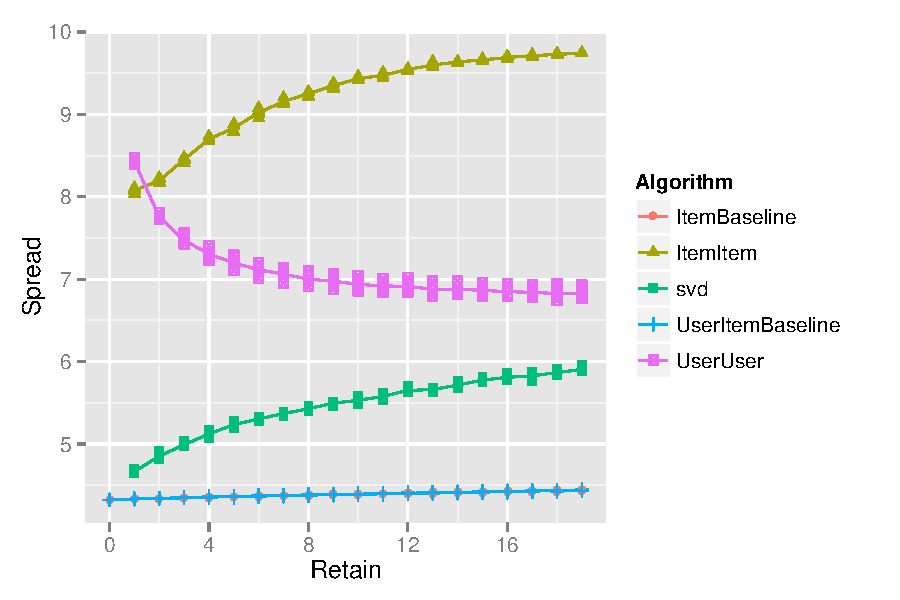
\includegraphics[width=\columnwidth]{../lenskit/target/analysis/topN_entropy.pdf}
\caption{caption}
\label{fig:spread}
\end{figure}









\section{Conclusions}

\section{Acknowledgements}
 \cite{harper2005economic}
 TODO:

\bibliographystyle{abbrv}
\bibliography{resources}  % sigproc.bib is the name of the Bibliography in this case

\end{document}
